%!TEX root=masterproef.tex

\chapter{Implementatie}
\label{chapter:implementatie}

\TODO

\inputminted[linenos,frame=lines,framesep=2mm,fontsize=\footnotesize]{js}{../src/foo-lang/examples/hello.foo}
\vspace{-5mm}
\captionof{listing}{Elementair voorbeeld in FOO-lang: hello.foo
  \label{lst:hello.foo}}

\section{Implementatiemiddelen}
\label{section:devel-tools}

\TODO

\subsection{Python}
\label{subsection:devel-python}

\TODO

\subsection{ANTLR}
\label{subsection:devel-antlr}

\TODO

\begin{figure}[ht]
  \centering
  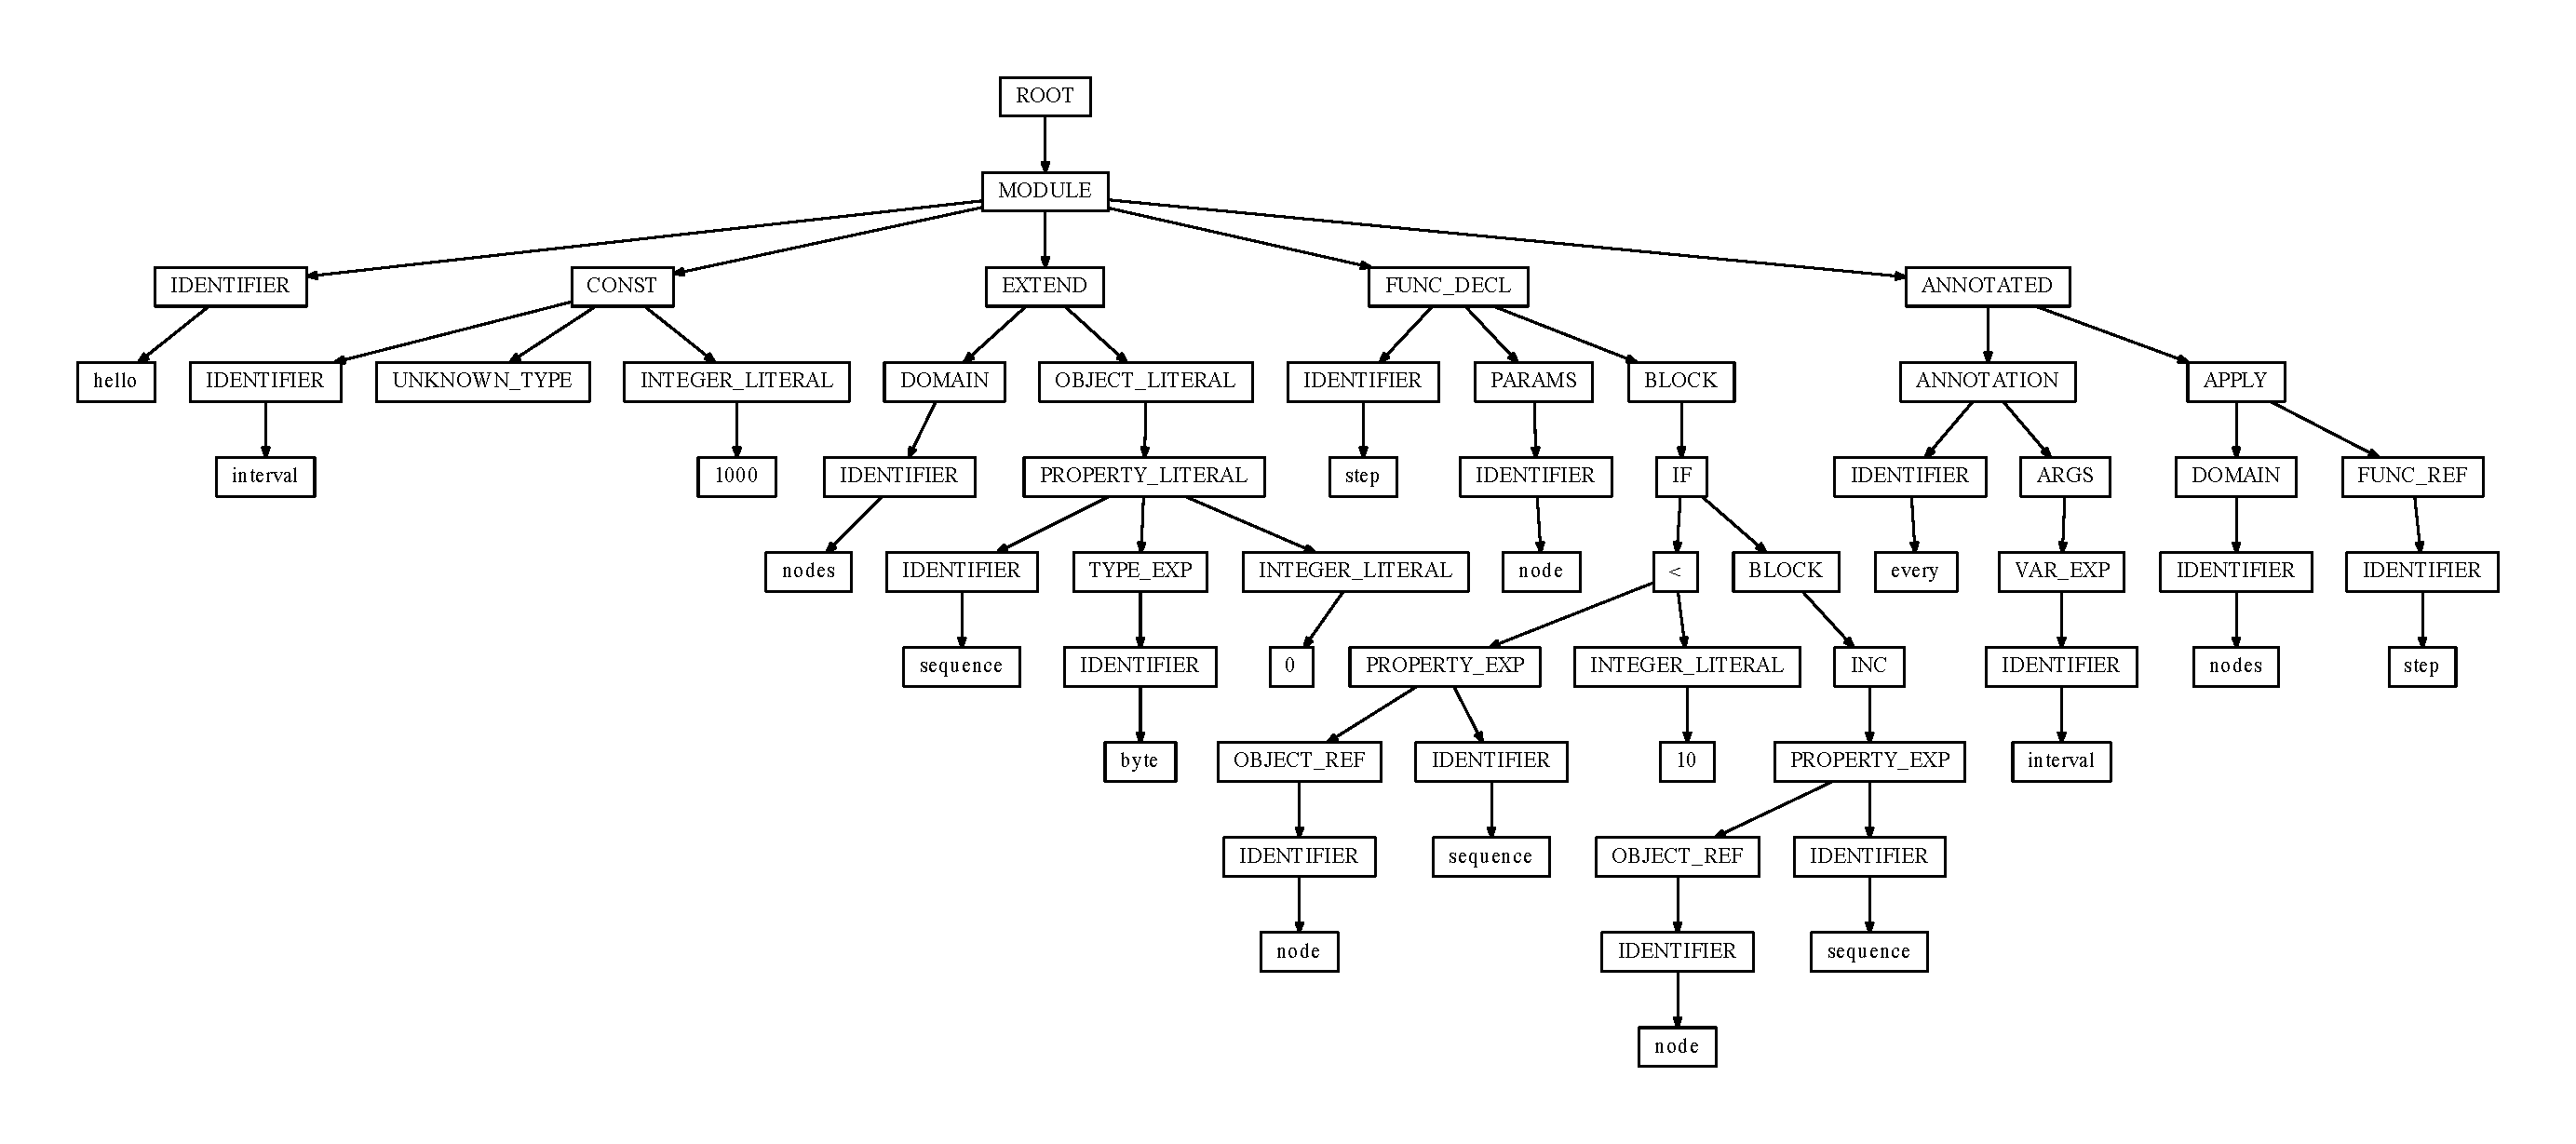
\includegraphics[width=\linewidth]{resources/hello_ast.pdf}
  \caption{Een AST}
  \label{fig:devel-ast}
\end{figure}
